\documentclass[compress]{beamer}
\usetheme{Warsaw}
\usecolortheme{whale}

\usepackage{amsmath}
\usepackage{url}
\usepackage{graphicx}
\usepackage{pgf}
\usepackage{tikz}
\usetikzlibrary{arrows,automata}
\usepackage[latin1]{inputenc}
\usepackage{verbatim}

%	\addtolength{\oddsidemargin}{-.5in}
%	\addtolength{\evensidemargin}{-.5in}
%	\addtolength{\textwidth}{0.75in}
%	\addtolength{\topmargin}{-1in}
%	\addtolength{\textheight}{1.75in}
\title{Predicting Web 2.0 Thread Updates}
\author{Shawn Tan}
\AtBeginSection[]
{
\begin{frame}{Table of Contents}
\tableofcontents[currentsection]
\end{frame}
}

\date{}
\begin{document}
\maketitle
\section{Introduction}

\begin{frame}{Motivation}
	\begin{itemize}
		\item Many sites with thread-based discussion features
		\item Users post product reviews, feedback
	\end{itemize}
	Obtaining such up-to-date information may be vital to companies.
\end{frame}

\begin{frame}{Crawling forums: The Naive way}
	One way of keeping the database \emph{fresh}, is to download pages at a frequent rate.

	However, forum sites are too large, with too many threads, incurring high bandwidth costs.
\end{frame}
\begin{frame}{Crawling forums: Estimating Future posts}
	Attempt to estimate future posts by learning from intervals between past posts.
	
% 	cite articles that use poisson distribution
\end{frame}
\begin{frame}{Our approach}
	Use the content as well to attempt to make a better prediction.
	\begin{itemize}
		\item Technical forum discussions
		\item Flame wars (e.g. Vim vs. Emacs)
	\end{itemize}
%For example, a thread in a technical forum about a Linux distribution may start out as a question. Subsequent questions that attempt to either clarify or expand on the original question may then be posted, resulting in a quick flurry of messages. Eventually, a more technically savvy user of the forum may come up with a solution, and the thread may eventually slow down after a series of messages thanking the problem solver. Suppose 10 days later, someone with a slight variation of the same problem posts on the thread again. A crawler solely on the age of the thread to determine its download rate of the thread may not update itself with the thread.
\end{frame}



%TODO:Bring to beginning and shorten to 1 or 2 sentences after the problem statement.
%as rate increase, timeliness become more important
% talk about consequences of naive method

\begin{frame}
Ideally, an incremental crawler of such user-generated content should be able to maintain a fresh content. 

However this
	\begin{enumerate}
		\item incur excessive costs when downloading un-updated pages
		\item raise the possibility of the web master blocking the requester's IP address.
	\end{enumerate}
\end{frame}

%Thus, we need a strategy of revisiting pages that will reduce the cost of downloading unchanged pages, while at the same time downloading them as soon as possible after it's update. 
%This year-long project proposes to use content-based features of a given thread to predict its next update time. We argue, that the content within the posts of the thread should be important in predicting the thread updates, and propose our approach to solving the problem.

\section{Related work}

\begin{frame}{Refresh policies for incremental crawlers}

Many works have used the Poisson distribution to model page updates.
	\begin{enumerate}
		\item Coffman et. al. 1997 analysed the theoretical aspects.
		\item Cho and Garcia-Molina trace the change history of 720,000 web pages collected over 4 months.
		\begin{enumerate}		
			\item Showed empirically that the Poisson process model closely matches the update processes found in web pages (Cho et. al. 1999)
			\item Proposed different revisiting or refresh policies (Cho et. al. 2003, Garcia-molina et. al. 2003)
		\end{enumerate}
		\item Also used in Tan et. al. 2007 and Wolf et. al. 2002. %elaborate!!!!
	\end{enumerate}
\end{frame}

\begin{frame}{Problems with Poisson}
	The Poisson distribution is memoryless, and in experimental results due to Brewington and Cybenko 2000, the behaviour of site updates are not. 
\end{frame}

\begin{frame}{Using Site-level Knowledge}
Yang et. al. 2009, attempted to resolve this by
	\begin{enumerate}
		\item Using the list structure of forum sites to infer a sitemap.
		\item Use a linear-regression model to predict when the next update to the thread will arrive. %elaborate!!!
	\end{enumerate}
\end{frame}


%Online forums and bulletins have a logical, hierarchical structure in their layout, which typically alerts the user to thread updates by putting threads with new replies at the very top of the thread index. Yang's work exploits this as well as their linear model to achieve a predicton of when to retrieve the pages.
%However, this is not so for comments found on blog sites or discussion threads in an e-commerce site about a certain product and the lack of these pieces of information may result in a poorer estimate, or no estimate at all.

%Our perspective is that the available content on the thread at the time of the retrieval should also be factored into the model used to predict the page updates. Next, we look at some of the related work pertaining to thread content.

%\begin{frame}{Should include?}
%Wang et. al \cite{Wang2011} did work in finding out linkages between forum posts using lexical chaining. They proposed a method to link posts using the tokens in the posts called $Chainer_{SV}$. While they do analyse the content of the individual posts, the paper does not make any prediction with regards to newer posts. The methods used to produce a numeric similarities between posts may be used as a feature to describe a thread in its current state, but incorporating this into our model is non-trivial.
%\end{frame}


%Kleinberg used Hidden Markov Models to predict ``bursts" in message arrival times \cite{Kleinberg2003}. In his running example, he used email messages, and used time between messages to estimate the states that produced the sequence. While the model may be able to predict what the state is for the next time interval, it does so using the history of message arrival times, and does not take into account the content within the messages themselves.


%One also cannot ignore the fact that social factors play a role when users interact in an online discussion. Granovetter's threshold model for social behaviour may also be useful in describing how the users behave as a whole.
\section{Preliminary Work}
\begin{frame}{Extracting Data}
	Collecting data from \url{http://forum.hardwarezone.com.sg} as our data set.
	\begin{itemize}
		\item User
		\item Timestamp
		\item Message body
	\end{itemize}
	
	Currently in raw HTML format, need to do preprocessing.

\end{frame}


\begin{frame}{Preliminary experiment}
We picked a few threads (more than 3 days):
\begin{enumerate}
	\item Computed time difference between posts $\Delta t$
	\item Sort posts by time difference
	\item Use median of $\Delta t$ as splitting point
	\item Tran a Naive Bayes classifier to classify posts into 2 categories:
	\begin{itemize}
		\item $\Delta t > 6$
		\item $\Delta t \leq 6$
	\end{itemize}
\end{enumerate}
\end{frame}

\begin{frame}{Results}

\begin{table}
	\label{table:naivebayesresults}
	\makebox[\textwidth][c]{
		\begin{tabular}{|l|c|c|c|}
			\hline
			Class				& Precision	& Recall	&	$F_1$ \\
			\hline
			$\Delta t \leq 6$	& 0.657 & 0.816 & 0.728 \\
			$\Delta t >    6$	& 0.682 & 0.483 & 0.565 \\
			\hline
		\end{tabular}
	}
	\caption{Naive Bayes classification results}
\end{table}
\begin{enumerate}
	\item 10-fold cross validation for results
	\item Low recall value for $\Delta t > 6$
\end{enumerate}
\end{frame}
\begin{frame}{User posting frequency}
\begin{figure}\label{sleepcycle}
\makebox[\textwidth][c]{\includegraphics[scale=0.4]{threadfreq.png}}
\end{figure}
\end{frame}


%The low recall for $\Delta t > 6$ may be due to a high number of overlapping terms in its vocabulary, causing a high number of false negatives. However, the results do suggest that there is some relationship between the content and $\Delta t$s that are less than or equal to 6 minutes. 


%We intend to implement the algorithm used in Yang et. al. \cite{Yang2009}, as a baseline to evaluate our system. However, since the algorithm uses the overall sitemap as additional information, only the linear regression model used to predict future incoming posts will be used. We will also use an SVM, trained using discretised time intervals and the extracted feature vectors.

%Compare with graph in paper... timeliness vs bandwith..
\begin{frame}{Evaluation metric}
To evaluate \emph{timeliness} of our algorithm we use the metric used in Yang et. al. 2009
\[T = \frac{1}{N} \sum^{N}_{i=1}\Delta t_i\]
\end{frame}



\begin{frame}{Observations}
	\begin{itemize}
		\item Content has some type of relationship with the update rates
		\item Thread update rates also dependent on users' sleep cycle
	\end{itemize}
\end{frame}
\begin{frame}{Thread States}
	\begin{itemize}
		\item Threads governed by probabilistic state machine
		\item Each state has an associated update rate, and set of observations (textual)
	\end{itemize}
\end{frame}
\begin{frame}{Hidden Markov Model}
	\begin{figure}[H]
		\begin{center}
	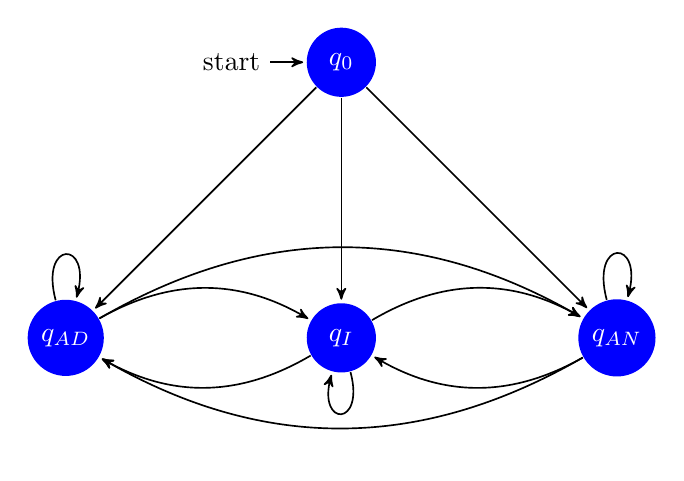
\begin{tikzpicture}[->,>=stealth',shorten >=1pt,auto,node distance=3.5cm,semithick]
	  \tikzstyle{every state}=[fill=blue,draw=none,text=white]

	  \node[initial,state] (q0)                    {$q_0$};
	  \node[state]         (IN) [below of=q0] {$q_I$};
	  \node[state]         (AD) [left of=IN] {$q_{AD}$};
	  \node[state]         (AN) [right of=IN] {$q_{AN}$};
	  \path (q0) edge              node {} (AD)
				 edge 			   node {} (AN)
				 edge 			   node {} (IN)
			(AD) edge [loop above] node {}(AD)
				 edge [bend left]  node {}(AN)
				 edge [bend left]  node {}(IN)
			(AN) edge [bend left]  node {}(AD)
				 edge [loop above] node {}(AN)
				 edge [bend left]  node {}(IN)
			(IN) edge [bend left]  node {}(AD)
				 edge [bend left]  node {}(AN)
				 edge [loop below] node {}(IN);
	\end{tikzpicture}

	\end{center}
		\caption{Modelling of a thread as a probabilistic automaton}\label{spaceship}
	\end{figure}
\end{frame}

\begin{frame}{State observations}
In the case of our thread content, possible observations include:
\begin{itemize}
	\item Average length of a post
	\item Word frequencies
	\item Time between posts
\end{itemize}
%Since new posts are more likely to be influenced by more recent posts, a form of weighted importance should be introduced, giving the later posts greater influence on the prediction.
\end{frame}

%\subsubsection{Lexical Chaining}
%One way to leverage the content in the thread might be to look at the post linkage structure. Lexical chaining gives a numerical relationship between each post in the thread. Analysing the time between these posts and the lexical chains, we may be able to predict, given the posts in the thread, when the next post may arrive.

%With these observations, the states that produce them, and the transitions between the states, given a thread, we may be able to produce a sequence of states that are highly likely to generate the observations. If we assume a certain rate of updates in each state, we would be able to calculate the expected interval between the last post and a future post.


%This is to account for the fact that a thread may be active, but the thread has a lack of activity, due to the fact that its' users are sleeping or working.



%We define active here as threads with a high post frequency, and inactive threads and as posts with low post frequency. Since our observations show that threads have different levels of post frequencies due to usage patterns consistent with user's sleep cycles and work commitment, we use 3 states in total to represent the state of a thread with more than 2 posts. A `day' state (represented by $q_{AD}$) and a `night' state (represented by $q_{ND}$). The inactive threads are represented by the state $q_I$
%Our initial model aims to incorporate these observations. A new thread (represented by $q_0$) which only has one post, may transition into either an active or inactive state (represented by $q_A$ respectively). We define active here as threads with high post frequency, and inactive threads as posts with low post frequency. Since our observations show that threads have different levels of post frequencies due to usage patterns consistent with user's sleep cycles, we use four states in total to represent the state of a thread with more than 2 posts, a `day' state and a `night' state (represented by $q_D,q_N$). These four states form a clique. Each of these states produce a set of observations that we can use to identify the state that a thread is in.

%The intuition behind this is the fact that active threads can transition to an inactive state, but the presence of a new post is able to spark off a new discussion within the thread, causing it to be an active thread again.

%The graphical representation of this automata is seen in Figure \ref{spaceship}.


%Our initial collection of data to identify changes in state for active threads to inactive threads do not show any observable patterns (See Figure \ref{nothing}). More data has to be collected and analysed before conclusions can be made. Statistics of textual content, along with data for a more complete set of threads may provide some insight to their behaviour.

%\section{Conclusion}
%A lot remains to be done over the next half of the academic year. More data for more sites with thread-based comment systems have to be collected in order to come up with a more general model. The baseline algorithms have to be implemented in order to perform evaluation. Most importantly, our algorithm has to be implemented and then evaluated against the baseline.



% use weka, do x-fold validation

%\begin{figure}
%	\includegraphics[scale=0.5]{view-comment.png}
%	\caption{Linear fit of Views vs Comments from forum.hardwarezone.com.sg}
%\end{figure}

\section{Work Plan}
\begin{frame}{Schedule}
\begin{center}
\scriptsize
\begin{tabular}{| l | l | c |}
	\hline
	Start date & End Date & Activity \\
	\hline
	%%%%%%%%%%%%%%%%%%%%%%%%%%%%%%%%%%%%%%%%%%%%%%%%%%%%%%%%%%%%%%%%%%%%%%
%%                                                                  %%
%%  This is a LaTeX2e table fragment exported from Gnumeric.        %%
%%                                                                  %%
%%%%%%%%%%%%%%%%%%%%%%%%%%%%%%%%%%%%%%%%%%%%%%%%%%%%%%%%%%%%%%%%%%%%%%
2012-05-07	&2012-05-11	&Implement feature extraction from threads\\
2012-05-14	&2012-05-18	&Collect more data from other forums\\
2012-05-21	&2012-05-25	&Implement baseline using classification algorithm (SVM)\\
2012-05-28	&2012-06-01	&Implement linear regression from Yang et. Al.\\
2012-06-04	&2012-06-08	&Implement and test HMM\\
2012-06-11	&2012-06-15	&Implement and test HMM\\
2012-06-18	&2012-06-22	&Implement and test HMM\\
2012-06-25	&2012-06-29	&Implement and test HMM\\
2012-07-02	&2012-07-06	&Implement and test HMM\\
2012-07-09	&2012-07-13	&Evaluation\\
2012-07-16	&2012-07-20	&Evaluation\\
2012-07-23	&2012-07-27	&Evaluation\\
2012-07-30	&2012-08-03	&Evaluation\\

	\hline
\end{tabular}
\end{center}
\end{frame}
\end{document}
